\documentclass[aspectratio=169]{beamer}
\setbeamertemplate{caption}[numbered]

\usepackage[utf8]{inputenc}
\usepackage{ragged2e}
\usepackage{multicol}
\usepackage{copyrightbox}
\usepackage{array}
\usepackage{booktabs}

\usetheme{Madrid}
\usecolortheme{default}

%------------------------------------------------------------
%This block of code defines the information to appear in the
%Title page
\title[Undergraduate Final Project] %optional
{Improving Kinship Verification using Face Age Transformation}

% \subtitle{A short story}

\author[Matheus Levi Rodrigues Aidano] % (optional)
{Matheus Levi Rodrigues Aidano\and \newline Advisor: Prof. Dr. Tiago Figueiredo Vieira}

\institute[] % (optional)
{
  Institute of Computing\\
  Universidade Federal de Alagoas
}

\date[December 13th] % (optional)
{Undergraduate Final Project, December 2024}

% \logo{
\includegraphics[height=1cm]{overleaf-logo}}

%End of title page configuration block
%------------------------------------------------------------



%------------------------------------------------------------
%The next block of commands puts the table of contents at the 
%beginning of each section and highlights the current section:

\AtBeginSection[]
{
  \begin{frame}
    \frametitle{Table of Contents}
    \tableofcontents[currentsection]
  \end{frame}
}
%------------------------------------------------------------


\begin{document}

%The next statement creates the title page.
\frame{\titlepage}


%---------------------------------------------------------
%This block of code is for the table of contents after
%the title page
\begin{frame}
\frametitle{Table of Contents}
\tableofcontents
\end{frame}
%---------------------------------------------------------

\section{Introduction}

\subsection{Motivation}

%---------------------------------------------------------------------------------------------------------------------------------------
\begin{frame}
\frametitle{Introduction}
Facial recognition systems are \textbf{essential} for biometrics and identification.

\begin{itemize}
    \item \textbf{Kinship verification} (KV) identifies family relationships through facial images.
    \item Aging significantly alters facial features, presenting a challenge for kinship models.
\end{itemize}

\vspace{0.4cm}
Face age transformation techniques have been improving recently, especially with the use of \textbf{GANs}

\begin{figure}[h]
    \centering
    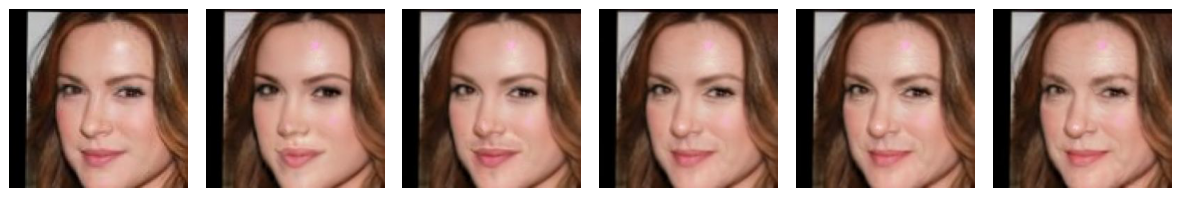
\includegraphics[scale=0.4]{Images/Img1.png}
    \caption{Facial aging transformation process}
    \label{fig:facial_aging_process}
\end{figure}

\end{frame}
%----------------------------------------------------------------------------------------------------------------------------------------

\begin{frame}
\frametitle{Motivation}

KV has implications in various domains, including social media, forensics, genealogy, and law enforcement.

\begin{itemize}
    \item Age-related facial changes obscure genetic similarities.
    \item Limited labeled datasets spanning diverse ages.
    \item Traditional methods often struggle to account for these \textbf{age-related changes}.
    \newline
\end{itemize}

\pause
In recent years, advances in deep learning, particularly GANs, have opened new avenues for addressing these challenges

\begin{itemize}
    \item Simulate \textbf{realistic} age progression and regression.
    \item Generate diverse age-transformed facial images.
    \item Improve model robustness to age-related variations.
\end{itemize}

\end{frame}

%---------------------------------------------------------------------------------------------------------------------------------------

\subsection{Objectives}

\begin{frame}
\frametitle{Objectives}
\textbf{General Objectives:} Enhance the accuracy and robustness of kinship verification models by integrating face age transformation techniques
\newline\newline
\textbf{Specific Objectives:}
\begin{itemize}
    \item Design a \textbf{GAN} to generate realistic age-transformed images while preserving identity;

    \item Augment kinship datasets with these images to improve model training;

    \item Develop a robust kinship verification model capable of handling age variation;

    \item Validate the approach using benchmark datasets and metrics;
\end{itemize}
\end{frame}

%---------------------------------------------------------------------------------------------------------------------------------------

\section{Theoretical Foundation and Literature Review}

\subsection{Neural Networks}

\begin{frame}
\frametitle{Neural Networks}
\justifying
Neural networks were first conceived in the mid-20th century, when Frank Rosenblatt established the concept of a \textbf{perceptron} \cite{rosenblatt1958perceptron}.

\vspace{0.4cm}
\begin{itemize}
    \item It has origins in \textbf{biological} systems and classic linear models
    \begin{itemize}
        \item Dendrites receive input signals from other neurons, process and transmit through the axon to other neurons;
        \item \textbf{Perceptrons} take input values, apply weights, and generate an output value;  
    \end{itemize}
\end{itemize}

\begin{equation}
z = w_1 x_1 + w_2 x_2 + \dots + w_n x_n + b
\end{equation}

\end{frame}

%---------------------------------------------------------------------------------------------------------------------------------------

\begin{frame}
\frametitle{Neural Networks}

\begin{columns}
    \begin{column}{0.5\textwidth}
    \justifying
     To improve neural networks capabilities, activation functions were invented, such as $\text{ReLU}(x) = \max(0, x)$ \cite{RELU}
    \newline

    \begin{itemize}
        \item The combined use of perceptrons created the \textbf{Neural Networks}
        \begin{itemize}
            \item Stacks of layers for hierarchical feature learning
            \item Backpropagation enables effective training
        \end{itemize}
    \end{itemize}
    
    \end{column}
    \hspace{0.1cm}

\begin{column}{0.4\textwidth}

    \begin{figure}[h]
    \centering
    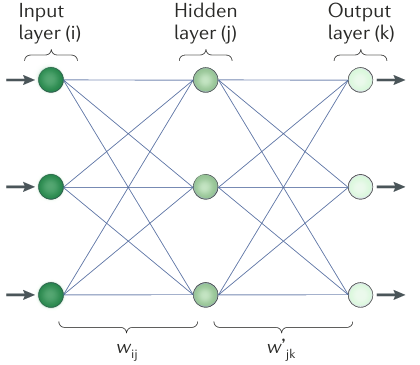
\includegraphics[scale=0.4]{Images/Img2.png}
    \caption{Example of a neural network. Source: \cite{neuron}}
    \label{fig:neuron_nn}
\end{figure}
    
\end{column}
\end{columns}
\end{frame}

%---------------------------------------------------------------------------------------------------------------------------------------

\begin{frame}
\frametitle{Convolutional Neural Networks}
\justifying

CNNs \cite{CNN} are a specialized type of neural network that is mainly used to process grid-like data, such as images.
    \begin{itemize}
        \item In each convolutional layer, a \textbf{convolutional operation} is performed along the input
        \item The convolution operation is used to slide the filter bank across the input, producing activations at each receptive field that combine to form a feature map
        \pause
        \item The job of a convolutional layer is to learn \textbf{kernels} that generate the most descriptive feature maps
    \end{itemize}

\begin{figure}[h]
    \centering
    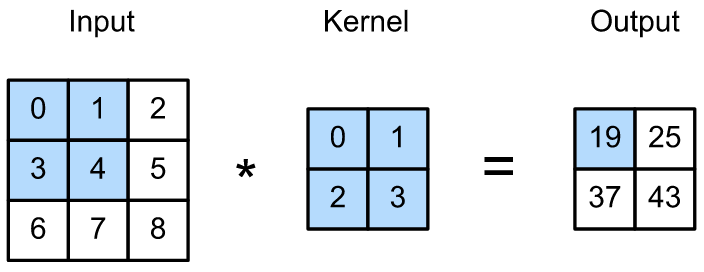
\includegraphics[scale=0.25]{Images/Img3.png}
    \caption{The convolution operation. Source \cite{convolution}}
    \label{fig:lenet5}
\end{figure}
\end{frame}

%---------------------------------------------------------------------------------------------------------------------------------------

\begin{frame}
\frametitle{Convolutional Neural Networks}
\justifying

CNNs \cite{CNN} consists mainly of two types of layers: 
    \begin{itemize}
        \item Convolutional layers capture spatial hierarchies: edges → textures → objects.
        \item Pooling (Subsampling) layers increase the level of abstraction through dimensionality reduction
    \end{itemize}


\begin{figure}[h]
    \centering
    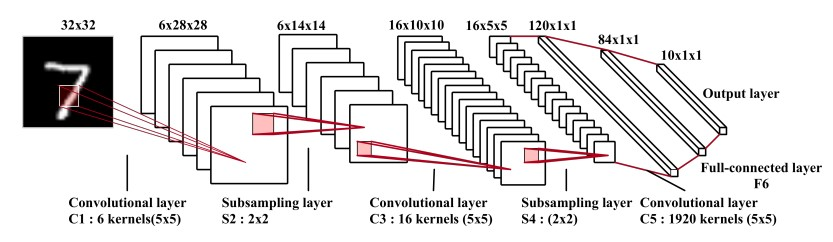
\includegraphics[scale=0.5]{Figures/Fig5.jpg}
    \caption{Example of a complete CNN architecture, LeNet-5. Source \cite{CNN}}
    \label{fig:lenet5}
\end{figure}
\end{frame}

%---------------------------------------------------------------------------------------------------------------------------------------

\begin{frame}
\frametitle{Residual Connections}

\begin{columns}
    \begin{column}{0.5\textwidth}
    \justifying
     Residual connections are an architectural feature in deep neural networks, which address the problem of \textbf{vanishing gradients} and degradation in performance as networks grow deeper \cite{resnet}
    \newline

    \begin{itemize}
        \item Residual connections allow information to \textbf{skip} layers, which can:
        \begin{itemize}
            \item Enable networks to learn without information loss
            \item Improve training stability and performance
        \end{itemize}
    \end{itemize}
    
    \end{column}
    \hspace{0.1cm}

\begin{column}{0.4\textwidth}

    \begin{figure}[h]
    \centering
    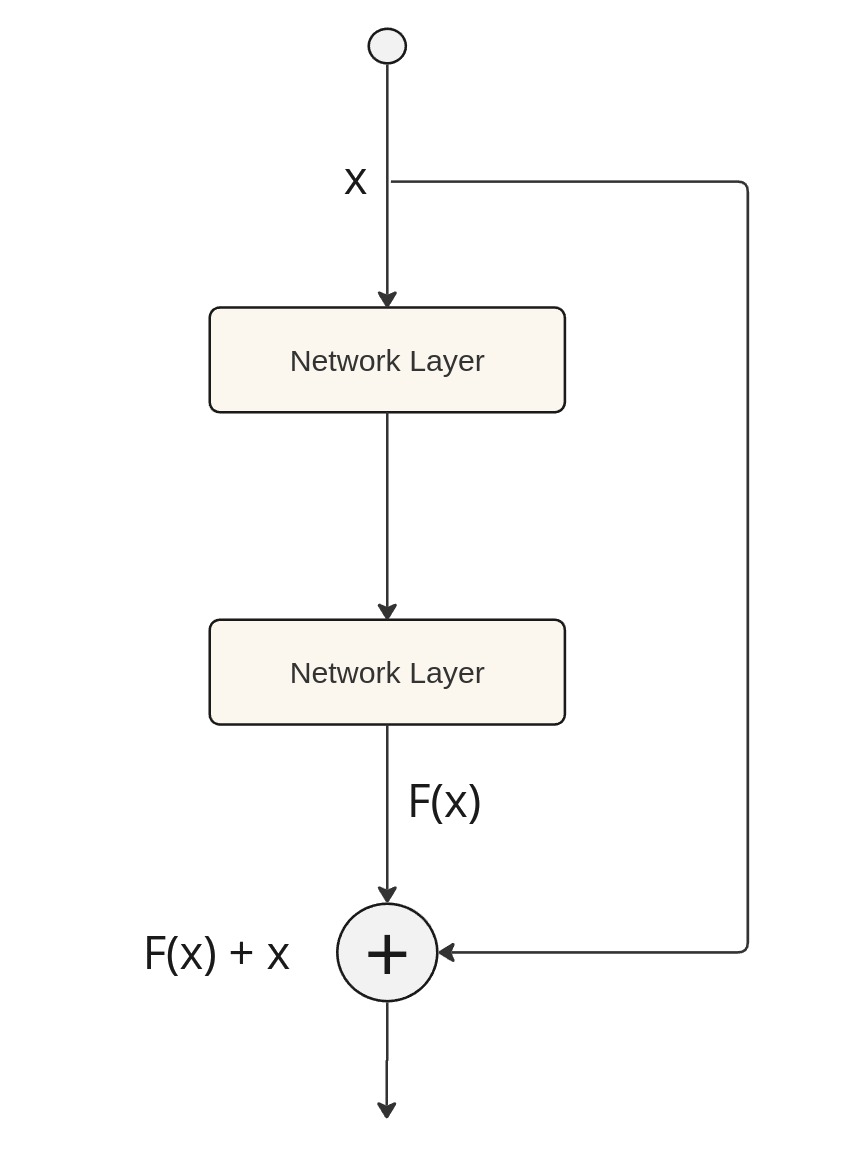
\includegraphics[scale=0.6]{Figures/Fig6.jpg}
    \caption{Residual block Illustration.}
    \label{fig:neuron_nn}
\end{figure}
    
\end{column}
\end{columns}
\end{frame}

%---------------------------------------------------------------------------------------------------------------------------------------

\subsection{Generative Adversarial Networks}

\begin{frame}
\frametitle{Generative Adversarial Networks}
\justifying

Generative Adversarial Networks (GANs) \cite{GAN} are a class of deep learning models designed for generative tasks, where the goal is to generate new data instances that resemble a given dataset
    \begin{itemize}
        \item Consists mainly in two components: Generator and Discriminator
        \item Adversarial Training pushes both components to improve
    \end{itemize}

\begin{block}{GANs objective function}
    \begin{equation}
        \min_G \max_D V(D, G) = \mathbb{E}_{x \sim p_\text{data}(x)}[\log D(x)] + \mathbb{E}_{z \sim p_z(z)}[\log(1 - D(G(z)))]
    \end{equation}
    where $x$ is the input image, $p_\text{data}$ is the true distribution and $p_z$ is the learned generator distribution
\end{block}

\end{frame}

%---------------------------------------------------------------------------------------------------------------------------------------

\begin{frame}
\frametitle{Generative Adversarial Networks}
\justifying

\begin{figure}[h]
    \centering
    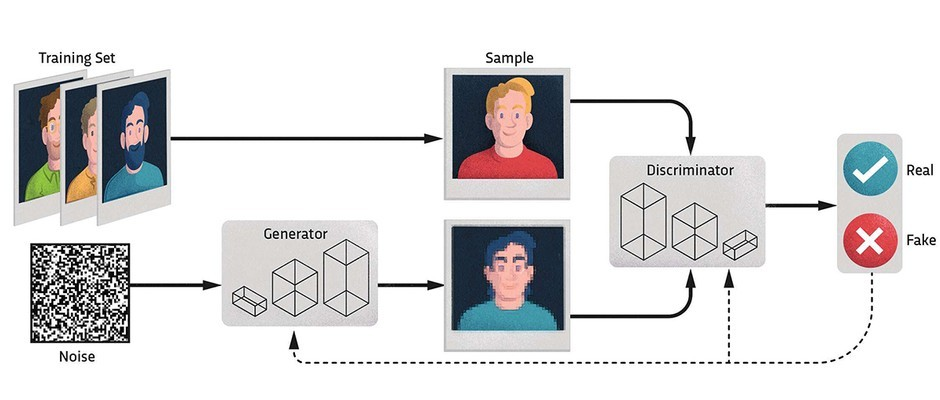
\includegraphics[scale=0.4]{Images/Img4.png}
    \caption{Visual representation of a Generative Adversarial Network. Source \cite{gan_linkedin}}
    \label{fig:lenet5}
\end{figure}
\end{frame}
%---------------------------------------------------------------------------------------------------------------------------------------

\subsection{Kinship Verification Overview}

\begin{frame}
\frametitle{Kinship Verification Overview}
\justifying

Kinship verification, is a task that aims to determine if two individuals have a \textbf{kin relationship} based on facial information

\begin{itemize}
        \item Human eyes have difficulties quantifying the similarity of two images from different people \cite{humanvsmachine}
        \item It has many potential applications, such as searching for missing children, border control, criminal investigations, etc. \end{itemize}

\end{frame}

%---------------------------------------------------------------------------------------------------------------------------------------

\begin{frame}
\frametitle{Problem Definition}
\justifying

Given a pair of faces $(X,Y)$, a kinship verification model should return a binary classification where 1 means that $X$ and $Y$ share a family relationship, and 0 otherwise.

\begin{itemize}
        \item Appropriate feature representations $(\phi(X), \phi(Y))$ are extracted from both images, and these features are compared using a form of similarity measurement, such as cosine similarity. \cite{siamesepaper}
\end{itemize}

\begin{figure}[h]
    \centering
    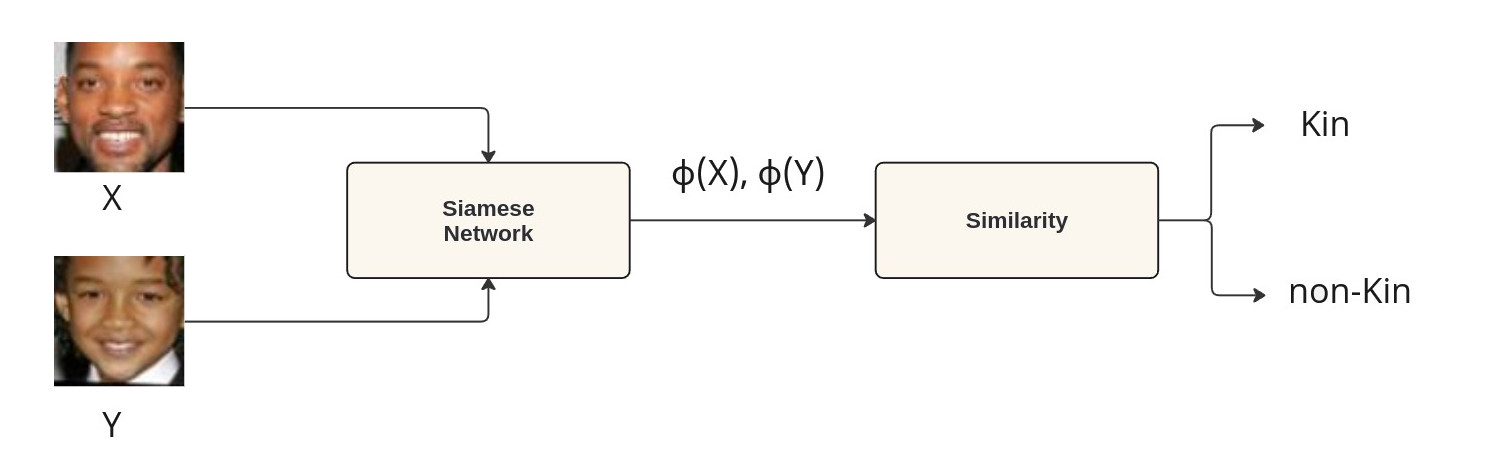
\includegraphics[scale=0.8]{Figures/Fig1_thin.jpg}
    \caption{General pipeline of Siamese Networks in Kinship Verification}
    \label{fig:lenet5}
\end{figure}
\end{frame}

%---------------------------------------------------------------------------------------------------------------------------------------

\begin{frame}
\frametitle{Main Challenges}
\justifying

KV is a more difficult problem than face recognition, since kinship pairs do not have the same identity but only share hidden genetic features \cite{debruine}.

\vspace{0.4cm}
\begin{itemize}
    \item Intrinsic Challenges
    \begin{itemize}
            \item Kinship pairs share subtle traits, unlike identical faces
            \item Aging and gender differences obscure familial similarities
            \item Positive pairs may look dissimilar; negative pairs may look alike
    \end{itemize}
\end{itemize}

\begin{itemize}
    \item Extrinsic Challenges
    \begin{itemize}
            \item Lighting, pose, and occlusion affect image quality
            \item Scarce labeled data for diverse age and kinship types
    \end{itemize}
\end{itemize}

\end{frame}

%---------------------------------------------------------------------------------------------------------------------------------------

\begin{frame}
\frametitle{Kinship Datasets}
\justifying

\begin{figure}[h]
    \centering
    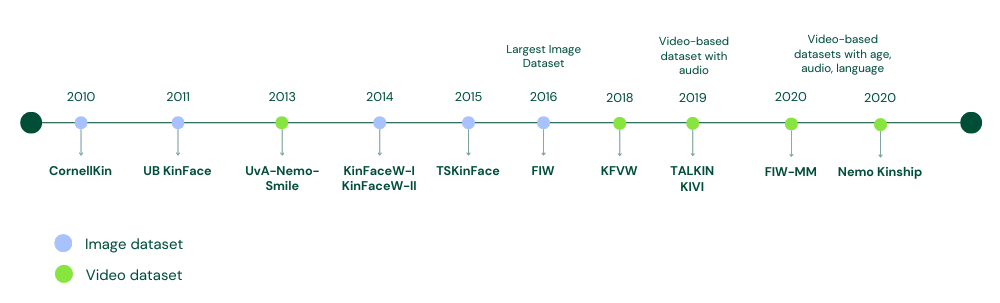
\includegraphics[scale=0.57]{Figures/Fig2.png}
    \caption{Development of representative kinship datasets. Source: \cite{asurveyonkinship}}
    \label{fig:lenet5}
\end{figure}
\end{frame}

%---------------------------------------------------------------------------------------------------------------------------------------

\begin{frame}
\frametitle{Existing Methods}
\justifying

\begin{itemize}
    \item Handcrafted Features
    \begin{itemize}
            \item Histogram of Gradients (HOG) \cite{hog}
            \item Local Binary Patterns (LBP) \cite{lbp}
            \item Scale-Invariant Feature Transform (SIFT) \cite{sift}
    \end{itemize}
\end{itemize}

\begin{itemize}
    \item Metric Learning
    \begin{itemize}
            \item Aim to learn a similarity function between pairs of images
            \item Neighborhood Repulsed Metric Learning (NRML) \cite{nrml}
    \end{itemize}
\end{itemize}

\begin{itemize}
    \item Deep Learning
    \begin{itemize}
            \item Learn feature representations from raw images
            \item \textbf{State-of-the-Art} in RFIW 2021 \cite{RFIW}
            \item Contrastive Learning
    \end{itemize}
\end{itemize}

\end{frame}

%---------------------------------------------------------------------------------------------------------------------------------------

\subsection{Facial Age Transformation Overview}

\begin{frame}
\frametitle{Facial Age Transformation Overview}
\justifying

\textbf{Facial age transformation} is a process that alters the appearance of a face to simulate aging or rejuvenation, while preserving the unique identity of the individual.

\begin{itemize}
        \item Applications in fields such as face recognition \cite{crossrecognition}, movie effects, and social entertainment. \cite{agetransapplications}
        \item Transformations must be highly accurate, as any deviation in identity or unrealistic aging can \textbf{reduce performance}
\end{itemize}

\end{frame}

%---------------------------------------------------------------------------------------------------------------------------------------

\begin{frame}
\frametitle{Problem Definition}
\justifying

Given an image $x_0$ of age $\alpha_0$ and a desired age $\alpha_1$ as input. The goal is to transform $x_0$ into the output $x_1 = G(x_0, \alpha_1)$, while maintaining age-unrelated characteristics.

\begin{itemize}
        \item In practical terms, identity preservation is \textbf{crucial} but difficult to maintain, as aging alters many facial features, such as wrinkles, skin texture, and facial structure.
        \item Factors such as genetics, lifestyle, health, and external conditions, such as environmental exposure, contribute to \textbf{different aging rates} \cite{agingrates}
\end{itemize}

\end{frame}

%---------------------------------------------------------------------------------------------------------------------------------------

\begin{frame}
\frametitle{Main Challenges}
\justifying

\begin{itemize}
    \item Identity Preservation
    \begin{itemize}
            \item Balancing realistic age progression with maintaining the individual’s \textbf{unique} traits
            \item Avoiding loss of key identity features such as facial structure, eyes, etc.
    \end{itemize}
\end{itemize}

\begin{itemize}
    \item Limited Data
    \begin{itemize}
            \item Few datasets with images of the same individual at multiple ages
            \item Diverse age representation across demographics is rare
    \end{itemize}
\end{itemize}

\begin{itemize}
    \item Visual Artifacts
    \begin{itemize}
            \item Generated images may suffer from blurriness, unnatural textures, or inconsistencies
            \item Larger \textbf{age gaps} amplify quality issues
    \end{itemize}
\end{itemize}


\end{frame}

%---------------------------------------------------------------------------------------------------------------------------------------

\begin{frame}
\frametitle{Age Datasets}
\justifying

\begin{table}[h!]
\centering
\begin{tabular}{|l|c|c|c|c|c|c|}
\hline
\textbf{Datasets} & \textbf{Images} & \textbf{Subjects} & \textbf{Age range} & \textbf{Average age} & \textbf{Year} \\ \hline
FG-NET          & 1002    & 82     & 0--69    & 15.84  & 2002 \\ 
MORPH2          & 553,349 & 13,672 & 16--77   & 32.69  & 2006 \\ 
CACD            & 163,446 & 2000   & 16--62   & 38.03  & 2014 \\ 
UTKFace         & 23,709  & --     & 0--116   & 33     & 2017 \\ 
AgeDB           & 16,488  & 568    & 1--101   & 50.3   & 2017 \\ 
FFHQ            & 70,000  & --     & --       & --     & 2019 \\ 
MRCD            & 64,965  & --     & 0--20    & --     & 2022 \\
B3FD            & 375,592  & 53,759     & 0--100    & --     & 2022 \\ \hline
\end{tabular}
\caption{Age Dataset summary}
\label{tab:ageTransDatasets}
\end{table}

\end{frame}

%---------------------------------------------------------------------------------------------------------------------------------------

\begin{frame}
\frametitle{Existing Methods}
\justifying

\begin{itemize}
    \item Traditional Methods
    \begin{itemize}
            \item Physical Model-Based: Simulate facial changes using biological parameters
            \item Prototype-Based: Use average faces for each age group to apply transformations.
    \end{itemize}
\end{itemize}

\begin{itemize}
    \item Deep Learning Methods
    \begin{itemize}
            \item Variational Autoencoders (VAEs) \cite{VAE}
            \begin{itemize}
                \item Encodes face into latent space for age manipulation.
                \item Limited realism in complex transformations.
            \end{itemize}
            \item Generative Adversarial Networks (GANs)
            \begin{itemize}
                \item \textbf{Conditional GANs} \cite{CGAN} such as IPCGAN \cite{IPCGAN}
                \item\textbf{Age-GAN}: Dual architecture for forward and reverse aging. \cite{ageGAN}
                \item \textbf{BiTrackGAN}: Cascaded CycleGAN for accurate, personalized aging. \cite{BiTrackGAN}
                \item \textbf{HRFAE}: Encoder-Decoder Generator for better image quality. \cite{HRFAE}
            \end{itemize}
    \end{itemize}
\end{itemize}

\end{frame}

%---------------------------------------------------------------------------------------------------------------------------------------
\section{Methodology}

\subsection{Data Preprocessing}

\begin{frame}
\frametitle{Data Preprocessing}
\justifying

The age transformation model was trained using \textbf{B3FD} \cite{B3FD} dataset
\begin{itemize}
    \item B3FD was filtered only for facial images of ages within the age range (20-70 years)
    \item Training with all the data could cause an \textbf{imbalance} in performance
    \item By choosing 2000 images per age, except for those that do not have enough, the final dataset used in the training had \textbf{93,325 images}
\end{itemize}

\begin{figure}[h]
    \centering
    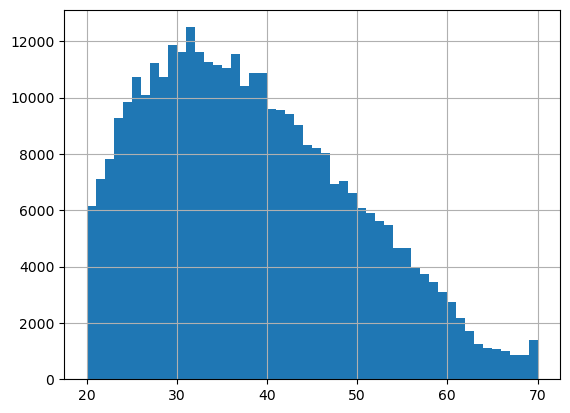
\includegraphics[scale=0.3]{Figures/Fig8.png}
    \caption{Age distribution of B3FD dataset}
    \label{fig:b3fdistribution}
\end{figure}

\end{frame}

%---------------------------------------------------------------------------------------------------------------------------------------

\subsection{Facial Age Transformation Model}

\begin{frame}
\frametitle{Facial Age Transformation Model}

The proposed approach for age transformation is an adaptation from \textbf{HRFAE} \cite{HRFAE} adjusted to low-resolution images.
\vspace{0.5cm}
\begin{itemize}
    \item Generator has an encoder-decoder architecture
    \item Age Encoder to insert age $\alpha_1$ into the network
    \item The discriminator focuses only on image fidelity
    \item The discriminator uses a \textbf{PatchGAN} framework \cite{patchGAN}
\end{itemize}

\end{frame}

%---------------------------------------------------------------------------------------------------------------------------------------

\begin{frame}
\frametitle{Facial Age Transformation Model}

\begin{itemize}
    \item The image encoder is constructed using convolutional layers and four residual blocks
    \item The age encoder is a simple fully connected layer with a sigmoid activation
\end{itemize}

\begin{figure}[h]
    \centering
    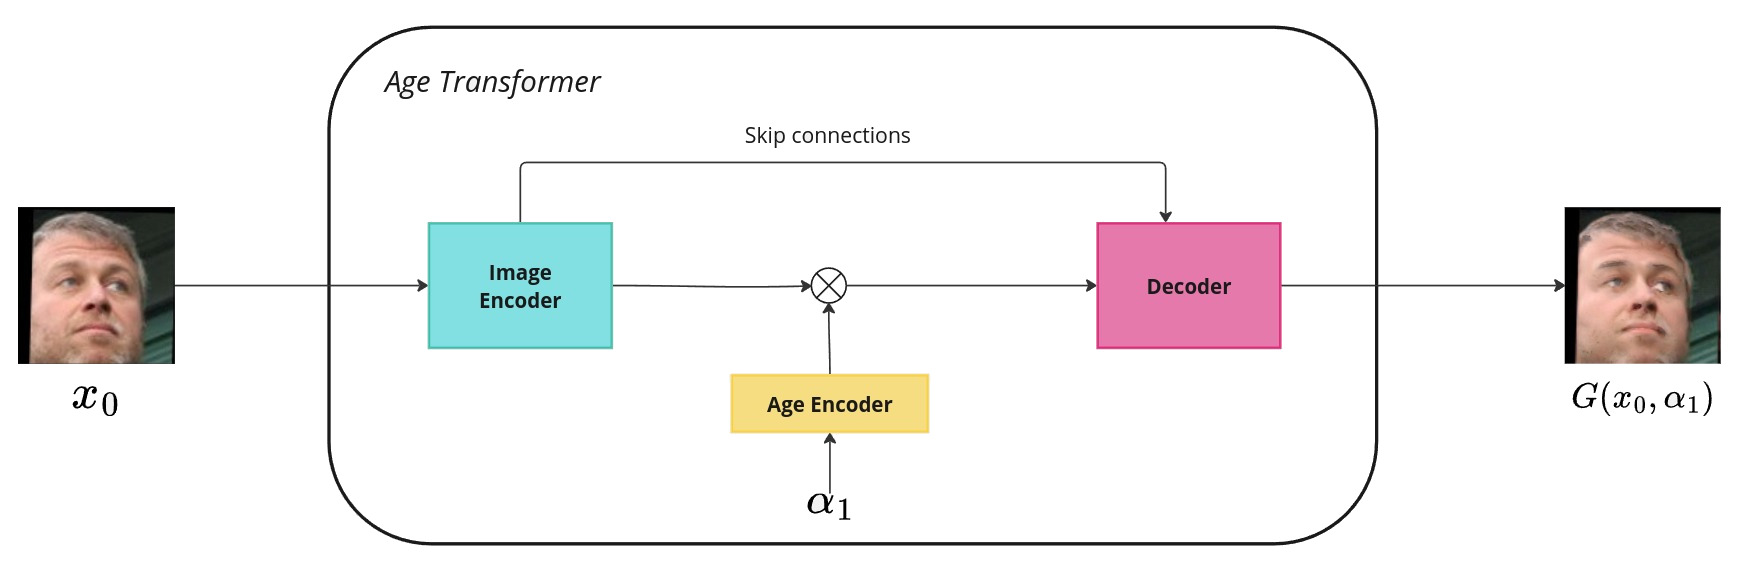
\includegraphics[scale=0.95]{Figures/Fig7.jpg}
    \caption{General Architecture of the age transformer generator}
    \label{fig:generator}
\end{figure}

\end{frame}

%---------------------------------------------------------------------------------------------------------------------------------------

\begin{frame}
\frametitle{Loss Functions}

\textbf{Reconstruction loss} encourages the model to generate an output that is identical to the input image when $\alpha_1 = \alpha_0$.

\begin{itemize}
    \item By minimizing this loss, the model learns to retain essential details and avoid unnecessary modifications
    \item This loss is crucial for preserving non-age-related features, such as identity, expression, and background detail
\end{itemize}

\begin{equation}
    \mathcal{L}_{\text{recon}} = \mathbb{E}_{\mathbf{x}_0 \sim p(x)} \left[ \| G(\mathbf{x}_0, \alpha_0) - \mathbf{x}_0 \|_1 \right].
\end{equation}

\end{frame}

%---------------------------------------------------------------------------------------------------------------------------------------

\begin{frame}
\frametitle{Loss Functions}

\textbf{Classification loss} ensures that the output transformed by age matches the specified target age, guiding the model to produce accurate age transformations. 

\begin{itemize}
    \item A pre-trained age classifier, denoted by $V$, is used to predict the age of the generated image on the one-hot vector $z_1$. 
    \item This is done by comparing the generated image's age $\alpha_0$ with the target age $\alpha_1$, helping the model accurately render age-relevant changes
\end{itemize}

\begin{block}{Classification Loss}
\begin{equation}
    \mathcal{L}_{\text{class}} = \mathbb{E}_{\mathbf{x}_0 \sim p(x)} \mathbb{E}_{\alpha_1 \sim q(\alpha | \alpha_0)} \left[ \ell(\mathbf{z}_1, V(G(\mathbf{x}_0, \alpha_1))) \right]
\end{equation}
where $p(x)$ represents the training image distribution over $X$ and $\ell$ denotes the categorical cross-entropy loss.
\end{block}

\end{frame}

%---------------------------------------------------------------------------------------------------------------------------------------

\begin{frame}
\frametitle{Loss Functions}

\textbf{Adversarial loss} is the main loss function, which guides the generator versus discriminator dynamic. For this, the LSGAN objective is adopted \cite{LSGAN}:

\vspace{0.4cm}
\begin{block}{Generator Loss}
\begin{equation}
    \mathcal{L}_{\text{GAN}}(G) = \mathbb{E}_{\mathbf{x}_0 \sim p(x)} \mathbb{E}_{\alpha_1 \sim q(\alpha | \alpha_0)} \left[ \left( D(G(\mathbf{x}_0, \alpha_1)) - 1 \right)^2 \right],
\end{equation}
\end{block}

\vspace{0.4cm}
\begin{block}{Discriminator Loss}
\begin{equation}
    \mathcal{L}_{\text{GAN}}(D) = \mathbb{E}_{\mathbf{x}_0 \sim p(x)} \mathbb{E}_{\alpha_1 \sim q(\alpha | \alpha_0)} \left[ \left( D(G(\mathbf{x}_0, \alpha_1))\right)^2 \right] + \mathbb{E}_{\mathbf{y} \sim p(x)} \left[ \left( D(\mathbf{y}) -1 \right)^2 \right]
\end{equation}
\end{block}

\end{frame}

%---------------------------------------------------------------------------------------------------------------------------------------

\begin{frame}
\frametitle{Loss Functions}

Finally, the \textbf{overall loss function} combines all three components:

\vspace{0.7cm}
\begin{equation}
    \mathcal{L} = \mathcal{L}_{GAN} + \lambda_{recon}\mathcal{L}_{recon} + \lambda_{class}\mathcal{L}_{class} 
\end{equation}
\vspace{0.7cm}

where $\lambda_{recon}$ and $\lambda_{class}$ are weights that balance the influence of each loss.

\end{frame}

%---------------------------------------------------------------------------------------------------------------------------------------

\subsection{Kinship Verification Model}
\begin{frame}
\frametitle{Kinship Verification Model}

The kinship verification model is a \textbf{Siamese neural network} that uses a contrastive loss framework \cite{sota21}.

Given a set $\mathcal{P} = \left\{ (x_i, y_i) \right\}_{i=1}^{n}$ where $n$ is the number of positive pairs sampled from different families, contrastive loss $L$ can be defined as:

\begin{block}{Contrastive Loss}
\begin{equation}
L = \frac{1}{2n} \sum_{i=1}^{n} \left[ L_c (x_i, y_i) + L_c (y_i, x_i) \right] 
\label{eq:contrastive}
\end{equation}

where

\begin{equation}
L_c (x_i, y_i) = - \log \frac{e^{s(x_i, y_i) / \tau}}{\sum_{j=1}^{n} e^{s(x_i, x_j) / \tau} + e^{s(x_i, y_j) / \tau}}
\label{eq:loss}
\end{equation}
\end{block}

\end{frame}

%---------------------------------------------------------------------------------------------------------------------------------------

\begin{frame}
\frametitle{Model Architecture}

\begin{figure}[h]
    \centering
    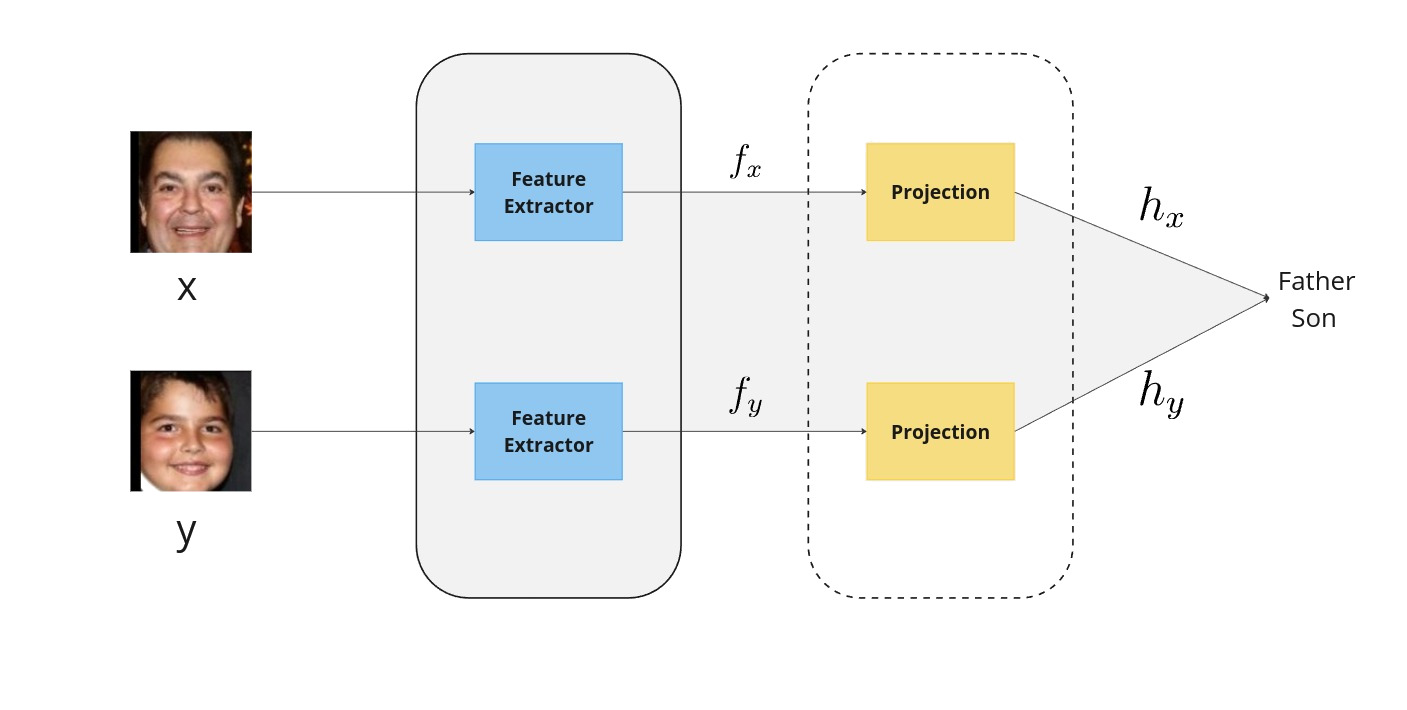
\includegraphics[scale=1.03]{Figures/Fig9.jpg}
    \caption{Kinship Model Training pipeline}
    \label{fig:kinshipmodel}
\end{figure}

\end{frame}

%---------------------------------------------------------------------------------------------------------------------------------------

\begin{frame}
\frametitle{Integration with Age Transformation}

The age transformation model was applied in \textbf{FIW} \cite{FIW} to generate images on 5 different ages, from 20 to 60 years. Then, this augmented dataset was used to train the kinship classification model.

\vspace{0.3cm}
\begin{itemize}
    \item The method chosen to utilize the age-transformed images was \textbf{random age sampling}.
    \item To increase the diversity of the dataset, randomly selected age-transformed images for each individual were added to training data.
    \item This approach aims to introduce variability, making the model more robust to age-related differences, and reduce over-fitting.
\end{itemize}

\end{frame}

%---------------------------------------------------------------------------------------------------------------------------------------

\subsection{Training}

\begin{frame}
\frametitle{Training}

\begin{table}[ht]
    \centering
    \begin{tabular}{ll}
        \hline
        \textbf{Parameter} & \textbf{Value(s)} \\
        \hline
        Epochs & 20 \\
        Batch size ($|B|$) & 4, 2 \\
        Image size & 128x128, 256x256 \\
        Optimizer & Adam \\
        Weight Decay & 0.0005 \\
        Learning Rate ($\alpha$) & 0.0001 \\
        $\lambda_{recon}$ & 10 \\
        $\lambda_{class}$ & 0.1 \\
        $\alpha_*$ & 25 \\
        \hline
    \end{tabular}
    \caption{Hyperparameters used in the age transformation model}
    \label{tab:agetrans_hyperparameters}
\end{table}

\end{frame}

%---------------------------------------------------------------------------------------------------------------------------------------

\begin{frame}
\frametitle{Training}

\begin{table}[ht]
    \centering
    \begin{tabular}{ll}
        \hline
        \textbf{Parameter} & \textbf{Value(s)} \\
        \hline
        Epochs & 80 \\
        Steps & 100 \\
        Batch size ($|B|$) & 25 \\
        Temperature ($\tau$) & 0.08 \\
        Optimizer & SGD \\
        Learning Rate ($\alpha$) & 0.0001 \\
        Momentum & 0.9 \\
        Threshold & 0.108667 \\
        \hline
    \end{tabular}
    \caption{Hyperparameters used in the kinship model}
    \label{tab:kinship_hyperparameters}
\end{table}

\end{frame}

%---------------------------------------------------------------------------------------------------------------------------------------

\section{Results and Discussions}

\begin{frame}
\frametitle{Results and Discussions}

\begin{figure}[h]
    \centering
    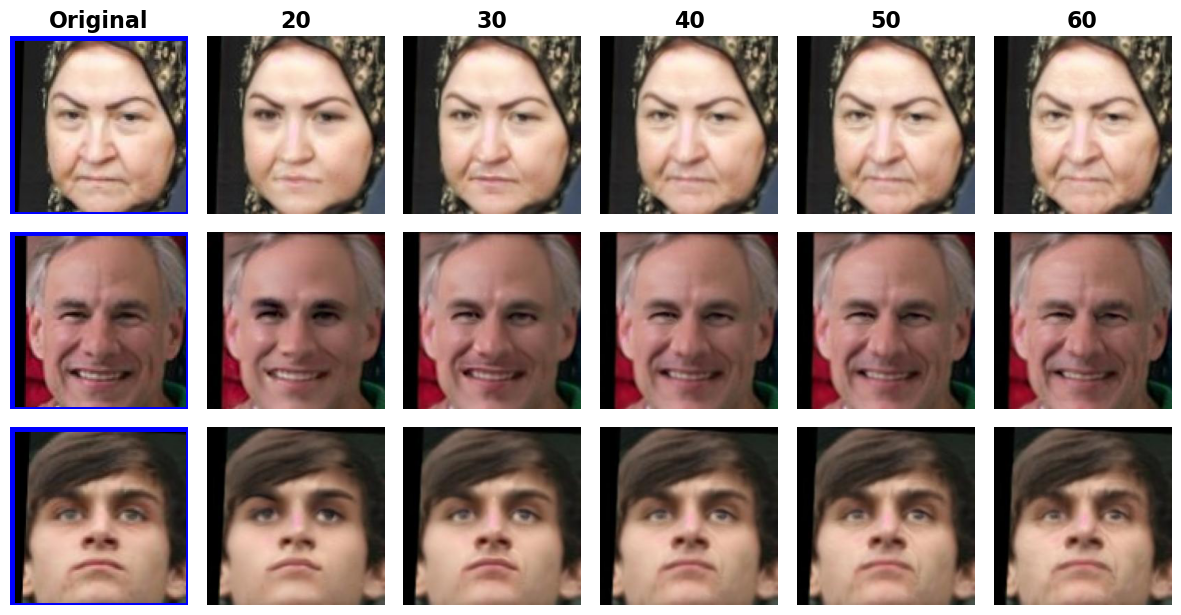
\includegraphics[scale=0.4]{Images/Img5.png}
    \caption{Age transformation results of 256x256 FIW images.}
    \label{fig:agetrans_examples}
\end{figure}
    
\end{frame}

%---------------------------------------------------------------------------------------------------------------------------------------

\begin{frame}
\frametitle{Results and Discussions}

\begin{columns}
    \begin{column}{0.3\textwidth}
        \begin{itemize}
            \item Ours has more consistent \textbf{visual fidelity}
            \item IPCGAN introduces noticeable \textbf{distortions} in some images
            \item Ours is more restrictive in terms of \textbf{identity preservation}
        \end{itemize}
    \end{column}

    \begin{column}{0.7\textwidth}
        \begin{figure}
            \centering
            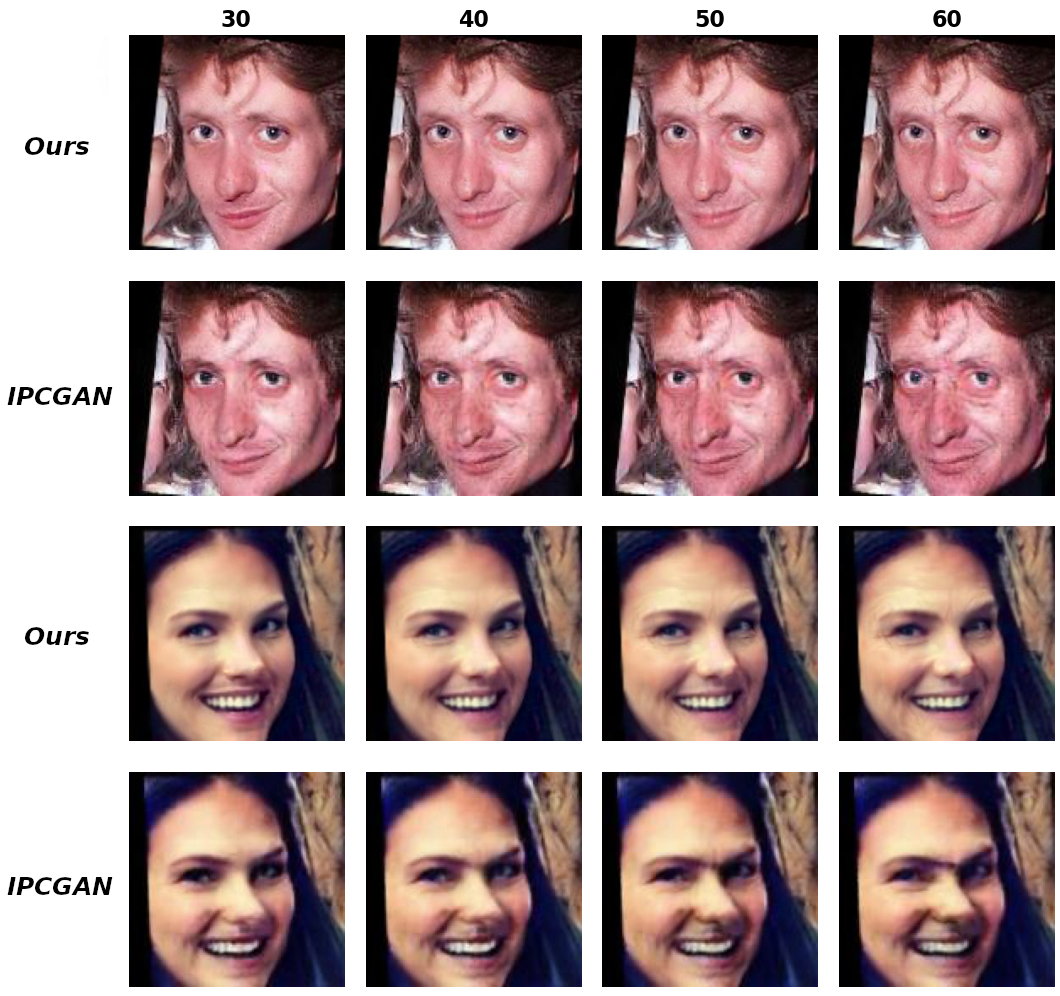
\includegraphics[scale=0.22]{Figures/fig11.png}
            \caption{Comparison with IPCGAN \cite{IPCGAN} on FIW.}
            \label{fig:examples_database_artificial}
        \end{figure}
    \end{column}
\end{columns}
    
\end{frame}

%---------------------------------------------------------------------------------------------------------------------------------------

\begin{frame}
\frametitle{Results and Discussions}

\vspace{0.4cm}
\begin{table}[h]
\centering
\begin{tabular}{|>{\centering\arraybackslash}m{3.5cm}|>{\centering\arraybackslash}m{2.0cm}|>{\centering\arraybackslash}m{2.0cm}|>{\centering\arraybackslash}m{2.0cm}|>{\centering\arraybackslash}m{2.0cm}|}
\hline
\textbf{Method} & \textbf{21-30} & \textbf{31-40} & \textbf{41-50} & \textbf{50+} \\ \hline
PAGAN  \cite{PAGAN}  & -     & 42.84 & 50.78 & \textbf{59.91} \\ \hline
AcGAN  \cite{acGAN}  & 25.92 & 36.49 & 40.59 & 47.88 \\ \hline
IPCGAN \cite{IPCGAN} & 46.15 & 55.41 & 53.86 & 55.64 \\ \hline
Ours                   & \textbf{62.9} & \textbf{58.10} & \textbf{57.36} & 55.64 \\ \hline
\end{tabular}
\caption{Aging accuracy comparison on different age groups.}
\label{tab:aging_accuracy}
\end{table}

\end{frame}

%---------------------------------------------------------------------------------------------------------------------------------------

\begin{frame}
\frametitle{Results and Discussions}

\begin{table}[ht]
    \centering
    \begin{tabular}{ll}
        \hline
        \textbf{Target image ($\alpha_1$)} & \textbf{Accuracy} \\
        \hline
        20 years & 86.65 \\
        30 years & 88.56 \\
        40 years & 89.57 \\
        50 years & 91.46 \\
        60 years & 93.10 \\
        \textbf{Average} & \textbf{89.87} \\
        \hline
    \end{tabular}
    \caption{Face recognition accuracy across all target images}
    \label{tab:recognition_accuracy}
\end{table}
\end{frame}

%---------------------------------------------------------------------------------------------------------------------------------------

\begin{frame}
\frametitle{Results and Discussions}

\begin{table}[ht]
    \centering
    \resizebox{\textwidth}{!}{
    \begin{tabular}{@{}lcccccccccccc@{}}
        \toprule
        \textbf{Method} & \textbf{BB} & \textbf{SS} & \textbf{SIBS} & \textbf{FD} & \textbf{MD} & \textbf{FS} & \textbf{MS} & \textbf{GFGD} & \textbf{GMGD} & \textbf{GFGS} & \textbf{GMGS} & \textbf{Average} \\ 
        \midrule
 Vuvko\cite{vuvko} & 0.80 & 0.80 & 0.77 & 0.75 & 0.78 & 0.81 & 0.74 & 0.78 & \textbf{0.76} & 0.69 & 0.60 & 0.780 \\
 DeepBlueAI\cite{deepblueAI} & 0.77 & 0.77 & 0.75 & 0.74 & 0.75 & 0.81 & 0.74 & 0.72 & 0.67 & \textbf{0.73} & \textbf{0.68} & 0.760 \\
 Ustc-nelslip\cite{ustc-nelslip} & 0.75 & 0.74 & 0.72 & \textbf{0.76} & 0.75 & \textbf{0.82} & 0.75 & \textbf{0.79} & \textbf{0.76} & 0.69 & 0.67 & 0.760 \\
 SupCL \cite{sota21} & 0.80 & \textbf{0.81} & \textbf{0.79} & 0.75 & 0.78 & 0.81 & 0.76 & 0.78 & 0.74 & 0.65 & 0.63 & 0.790 \\
 Ours & \textbf{0.81} & \textbf{0.81} & 0.78 & \textbf{0.76} & \textbf{0.79} & \textbf{0.82} & \textbf{0.77} & 0.77 & 0.70 & 0.68 & 0.62 & \textbf{0.792} \\
    \bottomrule
    \end{tabular}
    }
    \caption{Comparison of kinship verification accuracy across various methods.}
    \label{tab:accuracy_comparison}
\end{table}

\end{frame}

%---------------------------------------------------------------------------------------------------------------------------------------

\setbeamertemplate{bibliography entry article}{}
\setbeamertemplate{bibliography entry title}{}
\setbeamertemplate{bibliography entry location}{}
\setbeamertemplate{bibliography entry note}{}


\begin{frame}[allowframebreaks=0.85]{}
\frametitle{References}
    \nocite{*}
    \tiny
    \bibliographystyle{unsrt}
    \bibliography{references}
\end{frame}

\end{document}